\documentclass[letterpaper, reqno,11pt]{article}
\usepackage[margin=1.0in]{geometry}
\usepackage{color,latexsym,amsmath,amssymb,graphicx, float}
\usepackage{hyperref}

\hypersetup{
colorlinks=true,
linkcolor=magenta,
filecolor=magenta,
urlcolor=cyan,
}

\graphicspath{ {images/} }

\newcommand{\RR}{\mathbb{R}}
\newcommand{\CC}{\mathbb{C}}
\newcommand{\ZZ}{\mathbb{Z}}
\newcommand{\QQ}{\mathbb{Q}}
\newcommand{\NN}{\mathbb{N}}
\newcommand{\st}{\text{ s.t.}\ }

\begin{document}
\pagenumbering{arabic}
\title{ELEC 221 Homework 5}
\date{November 23, 2021}
\author{Xander Naumenko}
\maketitle

{\noindent\bf Question 1a.} From Fourier series definition, 

\[
    X(j\omega)=\int_{-\infty}^\infty x(t) e^{-j\omega t}dt=e^{-5j\omega}
\]

See figure \ref{fig:q1a} for the plot of the transform. 

\begin{figure}[htbp]
\centering
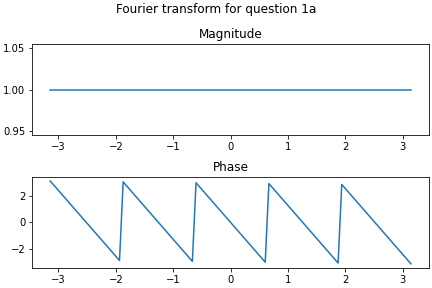
\includegraphics[width=\textwidth]{q1a.png}
\caption{Fourier transform for question 1a}
\label{fig:q1a}
\end{figure}

{\noindent\bf Question 1b.} Suppose that $x(t)$ is real and even. Then since $x(t)=x(-t)$, the imaginary part of $e^{-j\omega t}$ is odd and the real part is even, 

\[
    X(j\omega) = \int_{-\infty}^\infty x(t)e^{-j\omega t}dt=2\int_0^{\infty} x(t)\cos(\omega t)dt
\]

Clearly this is real as we are only integrating real numbers, and it is also even since the only $\omega$ dependence is in a $\cos$ which is even. 

{\noindent\bf Question 1c.} Assume $x(t)$ is real and odd. Again using the fact that the imaginary part of $e^{-j\omega}$ is odd and the real part is even, we get 

\[
    X(j\omega) = \int_{-\infty}^\infty x(t)e^{-j\omega t}dt=2j\int_0^\infty x(t)\sin(-\omega t)dt
\]

Note that the real part cancels since the product of two odd functions is even and the even real part goes to zero inside the integral. Since this is $j$ times an integral of a real function and the only $\omega$ dependence is $\sin$ which is odd, $X(j\omega)$ is also imaginary and odd. 

{\noindent\bf Question 1d.} Let $T=t-\tau$. Then $dT=dt$, and 

\[
    Y(j\omega) = \int_{-\infty}^\infty\int_{-\infty}^\infty x(\tau) h(T)e^{-j\omega \tau}e^{-j\omega T}d\tau dT
\]

By Fubini's theorem we can split the integral apart and we get 

\[
    Y(j\omega) = \int_{-\infty}^\infty x(\tau)e^{-j\omega\tau}d\tau=\int_{-\infty}^\infty h(T)e^{-j\omega T}dT=X(j\omega)H(j\omega)
\]

{\noindent\bf Question 2a.} Expanding and using the linearity of the integral we get 

\[
    X_3(j\omega) = \int_{-\infty}^\infty (\alpha x_1(t)+\beta x_2(t))e^{-j\omega t}dt=\alpha\int_{-\infty}^\infty x_1(t)e^{-j\omega t}dt+\beta\int_{-\infty}^\infty x_2(t)e^{-j\omega t}dt
\]
\[
    =X_1(j\omega)+X_2(j\omega)    
\]

{\noindent\bf Question 2b.} The integral of a delta function times a function is just the function evaluated at where the argument of the delta function is zero, so we get that 

\[
    \frac1{2\pi}\int_{-\infty}^\infty2\pi\delta(\omega-\omega_0)e^{j\omega t}d\omega=\frac{2\pi}{2\pi}e^{j\omega_0t}=e^{j\omega_0 t}    
\]

What we just showed is that the inverse fourier transform of $X(j\omega)=2\pi\delta(\omega-\omega_0)$ is $e^{j\omega_0t}$, and since the fourier transform is unique then the fourier transform of $e^{j\omega_0t}$ is $2\pi\delta(\omega-\omega_0)$. 

{\noindent\bf Question 2c.} Write out $x(t)$: 

\[
    x(t)=\sum_{k=-\infty}^\infty X_k e^{j2\pi tk/T}
\]

Using the definition of $X(j\omega)$, we have 

\[
    X(j\omega) = \int_{-\infty}^\infty \bigg(\sum_{k=-\infty}^\infty X_ke^{j2\pi kt/T}\bigg)e^{-j\omega t}dt
\]

Using the linearity of the FT that we found in part a: 

\[
    X(j\omega)=\sum_{k=-\infty}^{\infty} X_k \int_{-\infty}^\infty e^{-jt(\omega-2\pi k/T)}dt
\]

Applying the result of part b: 

\[
    X(\omega) = \sum_{k=-\infty}^\infty 2\pi X_k\delta\bigg(\omega-k\frac{2\pi}T\bigg)    
\]

Note that the question refers to $X_k$ as $\alpha_k$, these are the same in this case. 

{\noindent\bf Question 2d.} Plugging in the given coefficients to the definition of the fourier series we have 

\[
    s(t) = \sum_{k=1}^\infty \frac{X_k}2 e^{j\omega_0 kt}+\frac{X_k^*}2 e^{-j\omega_0 kt}=je^{j\pi t/4}-je^{-j\pi t/4}+2e^{j5\pi t/4}+2e^{-j5\pi t/4}
\]

% \[
%     s(t)=e^{j\pi t/4}-je^{-j\pi t/4}+2e^{j5\pi t/4}+2e^{-j5\pi t/4}
% \]

{\noindent\bf Question 2e.} Using our formula from part $c$, we get that the fourier transform is 

\[
    X(\omega) = \sum_{k=-\infty}^\infty 2\pi X_k\delta\bigg(\omega-k\frac{2\pi}T\bigg)=2\pi j\delta(\omega-\frac\pi4)-2\pi j\delta(\omega+\frac\pi4)+4\pi\delta(\omega-\frac{5\pi}{4})+4\pi\delta(\omega+\frac{5\pi}{4})
\]

The graph of this fourier transform can be seen in figure \ref{fig:q2e}. 

\begin{figure}[htbp]
\centering
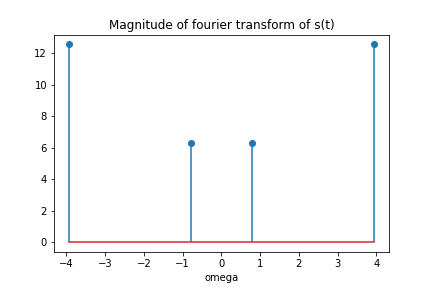
\includegraphics[width=\textwidth]{q2e}
\caption{Fourier transform of s(t) for question 2e. Note that the lines are actually delta functions}
\label{fig:q2e}
\end{figure}

{\noindent\bf Question 2f.} The filter output should filter out component frequencies that are not within it's band, which means the $k=\pm5$ components stay. Then the fourier coefficients are 

\[
    Y(j\omega)=X(j\omega)H(j\omega)=4\pi\delta(\omega-\frac{5\pi}4)e^{-j\omega}+4\pi\delta(\omega+\frac{5\pi}4)e^{-j\omega}
\]

\[
    =4\pi\delta(\omega-\frac{5\pi}4)e^{-j5\pi/4}+4\pi\delta(\omega+\frac{5\pi}4)e^{j5\pi/4}    
\]

\[
    \implies y(t)=2e^{j5\pi (t-1)/4}+2e^{-j5\pi (t-1)/4}
\]

{\noindent\bf Question 2g.} We already found the fourier transform of $y(t)$ in the previous part as $Y(j\omega)=X(j\omega)H(j\omega)$ as 

\[
    Y(j\omega)=4\pi\delta(\omega-\frac{5\pi}4)e^{-j5\pi/4}+4\pi\delta(\omega+\frac{5\pi}4)e^{j5\pi/4}    
\]

A plot of this transform can be seen in figure \ref{fig:q2g}. 

\begin{figure}[htbp]
\centering
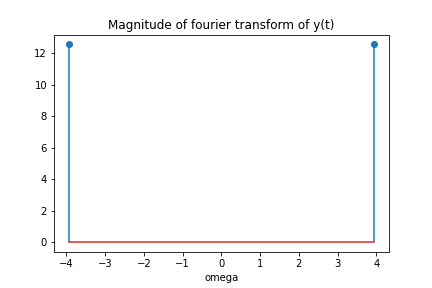
\includegraphics[width=\textwidth]{q2g.png}
\caption{Magnitude of the fourier transform of y(t). The band pass filter has filtered out the two lower frequency componenents. }
\label{fig:q2g}
\end{figure}


{\noindent\bf Question 3a.} See figure \ref{fig:q3a}

\begin{figure}[htbp]
\centering
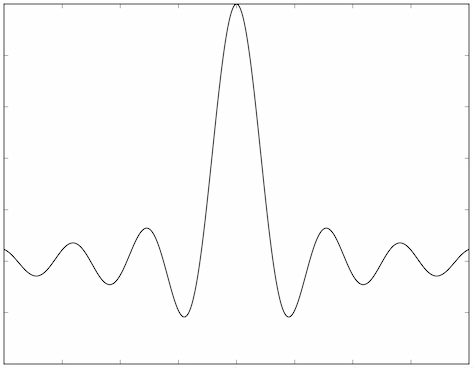
\includegraphics[width=\textwidth]{q3a}
\caption{Sinc function graphed}
\label{fig:q3a}
\end{figure}

{\noindent\bf Question 3b.} Using the integral table in the textbook, we see that 

\[
    X(j\omega)=\begin{cases}1&|\omega|<\frac\pi2\\0&\text{otherwise}\end{cases}
\]

Thus the sketch of $X(j\omega)$ can be seen in figure \ref{fig:q3b}. 

\begin{figure}[htbp]
\centering
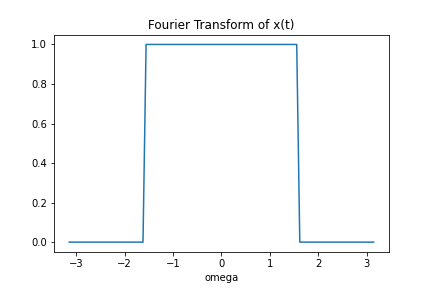
\includegraphics[width=\textwidth]{q3b}
\caption{Fourier transform for question 3b}
\label{fig:q3b}
\end{figure}

{\noindent\bf Question 3c.} Multiplication in time domain is the same as convolution in frequency domain, so 

\[
    W_1(j\omega)=\frac1{2\pi}\int_{-\infty}^\infty X(j\omega^\prime)X(j(\omega-\omega^\prime))d\omega^\prime=\begin{cases}1-|\frac{\omega}{\pi}|&|\omega|<\pi\\0&\text{otherwise}\end{cases}
\]

This convolution is easy to see visually, as the overlap between the two $X(j\omega)$ over the course of the convolution is a triangle. Next in the system we multiply by an impulse train, which corresponds with an fourier transform of 

\[
    P(\omega)=2\pi\sum_{k=-\infty}^\infty \delta(\omega-2\pi k)
\]

Again multiplication in time domain corresponds to convolution in the frequency domain, so we get 

\[
    W_2(j\omega) = \frac1{2\pi}(W_1*P)(j\omega)=\sum_{k=-\infty}^\infty W_1(j(\omega-2\pi k))
\]

Again this convolution was done graphically, since convolution with an impulse train causes the inputted signal to be repeated with the frequency of the impulse train. Next we multiply by $\cos(\pi t)$, which from the textbook's integral table has a fourier transform of $C(j\omega)=\pi(\delta(\omega-\pi)+\delta(\omega+\pi))$. Convolution with this has a net effect of translating the existing fourier transform by $\pi$ (this is because $W_2$ is already $2\pi$ periodic). Thus we have that the fourier transform for $w_3(t)$ is 

\[
    W_3(j\omega)=W_3(j(\omega-\pi))=\sum_{k=-\infty}^\infty W_1(j(\omega-\pi-2\pi k))
\]

Because of the linearity of the fourier transform, the final fourier transform of the output is then $W_2(j\omega+W_3(j\omega)$. This is 

\[
    Y(j\omega)=W_2(j\omega)+W_3(j\omega)=\sum_{k=-\infty}^\infty W_1(j(\omega-\pi-2\pi k))+\sum_{k=-\infty}^\infty W_1(j(\omega-2\pi k))
\]

Whereas before each of the triangle $W_1$ were seperate, now they overlap with their neighbours for exactly half of their width (since $W_1$ is $2\pi$ periodic and each copy of $W_1$ is only seperated by $\pi$). Thus between each copy we have two linear functions adding with opposite slopes which of course just adds to a constant, so the final fourier transform is 

\[
    Y(j\omega) = \frac12
\]

A graph of this (very simple) $Y(j\omega)$ can be seen in figure \ref{fig:q3c}. 

\begin{figure}[htbp]
\centering
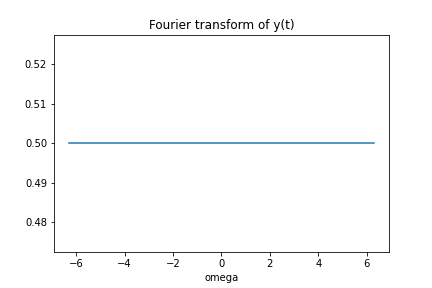
\includegraphics[width=\textwidth]{q3c}
\caption{Fourier transform for $y(t)$ in question 3c. }
\label{fig:q3c}
\end{figure}

{\noindent\bf Question 3d.} From the integral table in the textbook the inverse fourier transform of a constant is a delta function, so we get 

\[
    y(t)=\frac{\delta(t)}{2}
\]

The graph of this can be seen in figure \ref{fig:q3d}. 

\begin{figure}[htbp]
\centering
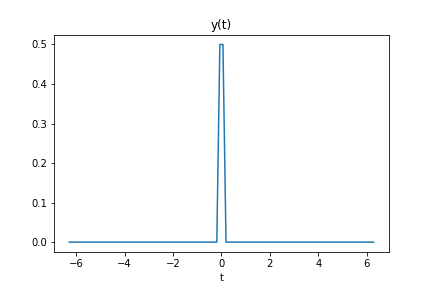
\includegraphics[width=\textwidth]{q3d}
\caption{y(t) for question 3d. Note that this is actually a delta function, and doesn't have a finite value. }
\label{fig:q3d}
\end{figure}

{\noindent\bf Question 3e.} As already stated above the frequency response of $h(t)$ is 

\[
    H(j\omega)=\begin{cases}1&|\omega|<\frac\pi2\\0&\text{otherwise}\end{cases}
\]

From the textbook the frequency response of the unit step function is

\[
    U(j\omega)=\frac1{j\omega}+\pi\delta(\omega)
\]

Convolution in time domain is multiplication in frequency domain, so 

\[
    Y(j\omega)=H(j\omega)U(j\omega)=\pi\delta(\omega)H(0)+\frac1{j\omega}H(j\omega)
\]

This is the exact form as a time domain integral, so we have that 

\[
    y(t)=\int_{-\infty}^t h(t^\prime)dt^\prime=\int_{-\infty}^t \frac{\sin(\frac{\pi t^\prime}2)}{\pi t^\prime}dt^\prime
\]

This is not an elementary integral to solve however, so we will leave it in this integral form. 

{\noindent\bf Question 3f.} See figure \ref{fig:q3f} for the plot. As expected, it exhibits ringing behaviour which manifests with oscillatory edges. This graph was produced by numerically integrating the final answer of the previous question, since no closed form expression in terms of elementary functions exists. 

\begin{figure}[htbp]
\centering
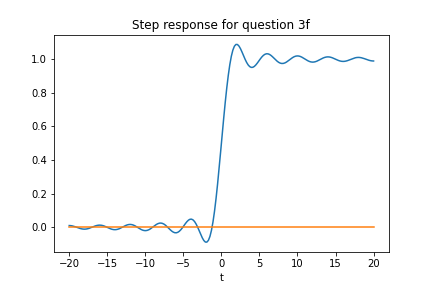
\includegraphics[width=\textwidth]{q3f}
\caption{Step response for h(t) for question 3f. }
\label{fig:q3f}
\end{figure}

{\noindent\bf Question 4a.} First we will find the frequency response. Taking the fourier transform of both sides, we have 

\[
    j\omega Y(j\omega)+Y(j\omega)=X(j\omega)
\]

\[
    H(j\omega)=\frac{Y(j\omega)}{X(j\omega)} = \frac1{1+\tau j\omega}
\]

For the impulse response, from the tables provided in the textbook we see that 

\[
    H(j\omega)=\frac1{a+j\omega}\implies h(t)=e^{-at}u(t)
\]

In our specific case, this means that 

\[
    H(j\omega)=\frac1\tau\frac1{\frac1\tau+j\omega}\implies h(t)=\frac1\tau e^{-\frac t\tau}u(t)
\]

{\noindent\bf Question 4b.} As we saw in question 3f, the step response is the integral of the impulse response. Thus 

\[
    y(t)=\int_{-\infty}^t h(t^\prime)dt^\prime=\int_{-\infty}^t\frac1\tau e^{-t^\prime/\tau}u(t^\prime)dt^\prime=\int_{0}^t\frac1\tau e^{-t^\prime/\tau}dt^\prime=1-e^{-t^\prime/\tau}\bigg|_0^t=1-e^{-t/\tau}
\]

As expected at $t=\tau$, $y(t)=1-\frac1e$. This step response can be seen in figure \ref{fig:q4b}. In this case ringing does not occur, unlike question 4f. 

\begin{figure}[htbp]
\centering
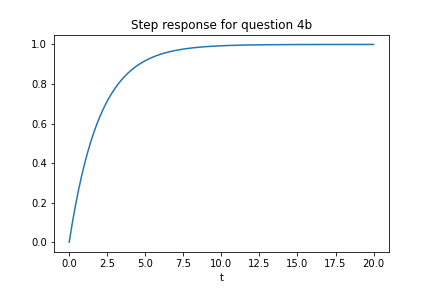
\includegraphics[width=\textwidth]{q4b}
\caption{Step response for question 4b. Note that ringing does not occur. For this graph an arbitrary $\tau=2$ was used. }
\label{fig:q4b}
\end{figure}

{\noindent\bf Question 4c.} The plot of the frequency response we found in part a can be seen in figure \ref{fig:q4c}. As expected, it is a rather poor low pass filter but is one nonetheless. 

\begin{figure}[htbp]
\centering
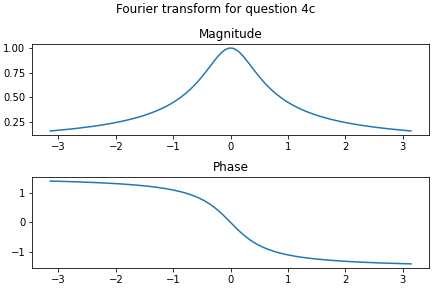
\includegraphics[width=\textwidth]{q4c}
\caption{Frequency response for question 4c, again with $\tau=2$. }
\label{fig:q4c}
\end{figure}

{\noindent\bf Question 4d.} Expanding out the definition of the frequency response for $-j\omega$ and $j\omega$, we have 

\[
    H(j\omega)=\int_{-\infty}^\infty x(t)e^{-j\omega t}dt=\int_{-\infty}^\infty x(t)cos(\omega t)dt+i\int_{-\infty}^\infty x(t)\sin(\omega t)dt
\]
\[
    H(-j\omega)=\int_{-\infty}^\infty x(t)e^{j\omega t}dt=\int_{-\infty}^\infty x(t)cos(\omega t)dt-i\int_{-\infty}^\infty x(t)\sin(\omega t)dt
\]

Since by hypothesis the signal $x(t)$ is real, then the integrals are all real, and by inspection of the terms we have that $H(j\omega)=H(-j\omega)^*$. Using this formula all one needs is the frequency response for positive $\omega$ and the negative parts can be found by just taking the conjugate. 

{\noindent\bf Question 4e.} Using one of the fundamental properties of an LTI, we know that 

\[
    Y(j\omega)=H(j\omega)X(j\omega)
\]

Applying logarithm rules, we get that 

\[
    \log Y(j\omega)=\log(H(j\omega)X(j\omega))=\log H(j\omega)+\log X(j\omega)
\]

This was what we needed to show so we're done. 

{\noindent\bf Question 4f.} See figure \ref{fig:q4f}. $\tau=2$ and $\tau=0.5$ are plotted. 

\begin{figure}[htbp]
\centering
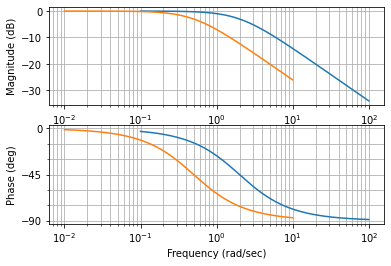
\includegraphics[width=\textwidth]{q4f}
\caption{Bode plot for question 4f. Orange line is $\tau=2$, blue line is $\tau=0.5$}
\label{fig:q4f}
\end{figure}

{\noindent\bf Question 4g.} When $\omega\tau\ll1$, then we have 

\[
    20\log_{10}|H(j\omega)|=20\log_{10}|\frac1{1+j\omega\tau}|\approx 20\log_{10}\frac{1}{1}=0
\]

For $\omega\tau\gg1$, expand to get 

\[
    20\log_{10}|H(j\omega)|=20\log_{10}|\frac1{1+j\omega\tau}|=-20\log_{10}|1+j\omega\tau|\approx-20\log_{10}|j\omega\tau|
\]

\[
    =-20\log_{10}\omega-20\log_{10}\tau
\]

This is what was required to show so we're done. 

{\noindent\bf Question 4h.} See figure \ref{fig:q4h}. The value of the graph at $omega=\frac1\tau$ is approximately $3$dB. This makes sense as the magnitude has been reduced by 3dB. 

\begin{figure}[htbp]
\centering
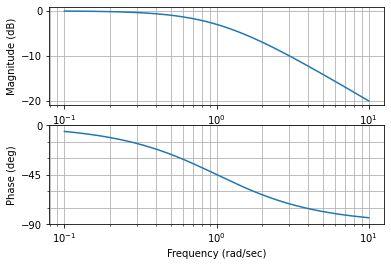
\includegraphics[width=\textwidth]{q4h}
\caption{Generalized bode plot. In this case $\tau=1$ but can be scaled to anything. }
\label{fig:q4h}
\end{figure}

{\noindent\bf Question 4i.} Again taking the fourier transform of both sides we get 

\[
    (j\omega)^2Y(j\omega)+2\zeta\omega_n(j\omega) Y(j\omega)+\omega_n^2Y(j\omega)=\omega_n^2X(j\omega)
\]

\[
    H(j\omega)=\frac{Y(j\omega)}{X(j\omega)}=\frac1{(j\omega/\omega_n)^2+2\zeta(j\omega/\omega_n)+1}
\]

{\noindent\bf Question 4j.} See figure \ref{fig:q4j}. 

\begin{figure}[htbp]
\centering
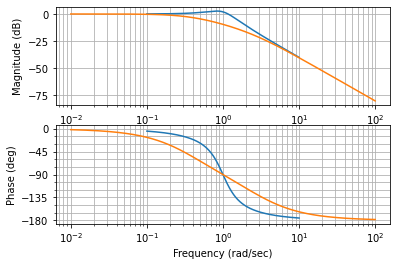
\includegraphics[width=\textwidth]{q4j}
\caption{Bode plot of frequency response. Blue line is $\zeta=0.4$, orange line is $\zeta=1.5$. }
\label{fig:q4j}
\end{figure}

{\noindent\bf Question 4k.} For $\omega\ll\omega_n$, we have 

\[
    20\log_{10}|H(j\omega)|=20\log_{10}\frac1{(j\omega/\omega_n)^2+2\zeta(j\omega/\omega_n)+1}\approx 20\log_{10}\frac11=0
\]

For $\omega\gg\omega_n$, we instead have 

\[
    20\log_{10}|H(j\omega)|=20\log_{10}|\frac1{(j\omega/\omega_n)^2+2\zeta(j\omega/\omega_n)+1}|=-20\log_{10}|((j\omega/\omega_n)^2+2\zeta(j\omega/\omega_n)+1)|
\]

\[
    \approx-20\log_{10}|(j\omega/\omega_n)^2|=-40\log_{10}\omega+40\log_{10}\omega_n
\]

As can be seen now the slope has become $40$, which means that it is a better low pass filter than parts a-g. The result is also confirmed by the bode plots produced in parts i and j, since they have the correct slope. 


\end{document}